\documentclass[12pt]{article}
\usepackage[utf8]{inputenc}
\usepackage{amsmath, amsfonts, amssymb}
\usepackage[a4paper, margin=1in]{geometry}
\usepackage{varwidth}
\usepackage{graphicx}

\title{Random Variables and Stochastic Process (AI5030)}
\author{Soumyajit Chatterjee\\AI22MTECH02005 }


\begin{document}

\maketitle

\section*{Question 55 Dec (2018)}
Let $(X_1, Y_1), (X_2, Y_2), (X_3, Y_3) \dotsc (X_n, Y_n)$ be n independent observations from a distribution. Let r$_p$ be the product moment correlation coefficient and r$_s$ be the rank correlation coefficient computed based on n observations. Which of the following statements is correct. 

1. r$_p \geqslant 0$ implies r$_s \geqslant 0$

2. r$_s \geqslant 0$ implies r$_p \geqslant 0$

3. r$_p = 1 $ implies r$_s = 1$

4. r$_s = 1 $ implies r$_p = 1$

\section*{Solution}

\textbf{Theoretical proof}

\noindent The correlation coefficient for a bi-variate dataset with the independent vector as X and dependent vector as Y is given by

$$
\rho = \dfrac{cov(X,Y)}{var(X) * var(Y)}
$$

\vspace{4mm}
Where the covariance of X, Y in vector form is given as:

$$
\text{cov(X,Y)} = \text{E}[(X-\overline{X})^T \, (Y-\overline{Y})]
$$

\vspace{4mm}
Where the variance of X in vector form is given as:
$$
\text{var(X)} = \text{E}[(X-\overline{X})^T \, (X-\overline{X})]
$$

\noindent The product moment correlation coefficient r$_p$ is also given as:

$$
\rho = \dfrac{cov(X,Y)}{var(X) * var(Y)}
$$

\vspace{2mm}

\noindent The assumption made while calculating r$_p$ is that there exists some linear relation among the X and Y variables in the data.

\vspace{3mm}

\noindent Here, linear relation means a straight line relationship exists between X and Y.

\noindent The rank correlation coefficient r$_s$ is given as:

$$
\rho = \dfrac{cov(R(X),R(Y))}{var(R(X)) * var(R(Y))}
$$

\vspace{3mm}

\noindent Where R( ) returns the rank/index of the sorted data as appearing in the dataset. 

\noindent The assumption made while calculating r$_s$ is that there exists some monotonic relation among the X and Y variables in the data.

\vspace{3mm}

\noindent Here, monotonic relation means some increasing relationship exists between X and Y. Example, Y can be increasing linearly with X, Y can be increasing parabolically with X, Y can be increasing exponentially with X.

\vspace{3mm}

\noindent Without loss of generality we can say that a linear function is a subset of monotonic functions.

\vspace{3mm}

\noindent Therefore, r$_p \geqslant 0$ means positive linear correlation which means as X increases, Y also increases linearly.

\vspace{3mm}

\noindent r$_s \geqslant 0$ means positive monotonic correlation which means as X increases, Y also increases monotonically.

\noindent If a function increases linearly it must be increasing monotonically as well as linear functions are a subset of monotonic functions.

\vspace{3mm}

\noindent Therefore, from the above logic option (1) and option (3) are correct i.e r$_p \geqslant 0$ implies r$_s \geqslant 0$ and r$_p = 1$ implies r$_s = 1$ which is also a case of option (1).

\vspace{3mm}

\noindent \textbf{Proof From simulation}
\begin{figure}[h]
    \centering
    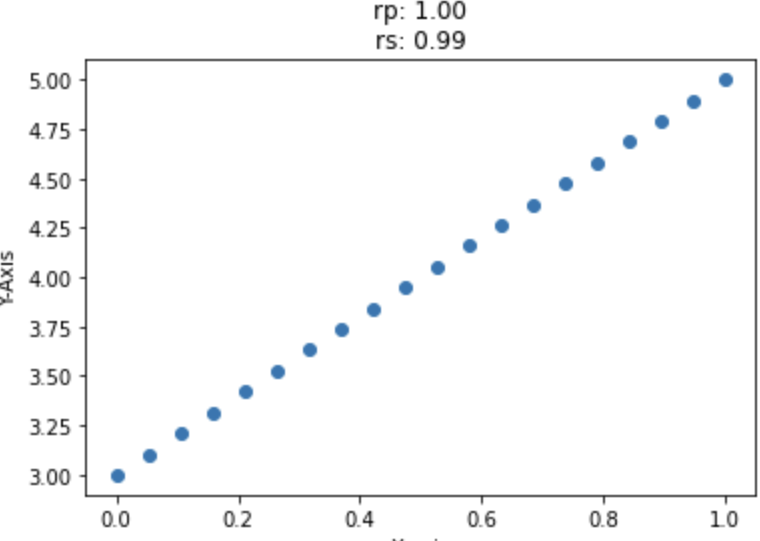
\includegraphics[width=0.7\textwidth]{c3.png}
    \caption{Linear Data}
    \label{fig:c3}
\end{figure}

\vspace{3mm}
\noindent From the above plot we can see that since data is linear, r$_p$ is positive and r$_s$ is also positive and both of them are equal to 1 justifying option (1) and option(3) that for linear data r$_p$ implies r$_s$.
\clearpage

\begin{figure}[h]
    \centering
    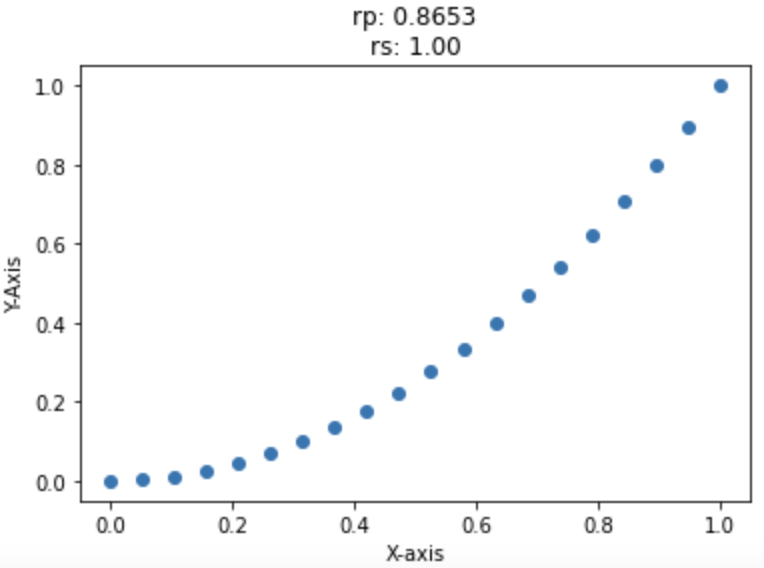
\includegraphics[width=0.7\textwidth]{c4.png}
    \caption{Exponential Data}
    \label{fig:c4}
\end{figure}

\vspace{3mm}

\noindent From the above plot we can again see that if r$_p$ is positive then r$_s$ is also positive. But since data is not linear but simply monotonic, therefore r$_p$ is not 1 but r$_s$ is still 1 as r$_s$ assumes any monotonic relation between the data points.

\vspace{3mm}
\noindent Therefore, r$_p = 1$ implies r$_s = 1$ but not the other way around as every linear function is monotonic but every monotonic function is not linear. Therefore this plot also justifies option (1) and option (3).  

\end{document}